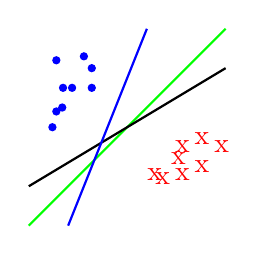
\begin{tikzpicture}[scale=0.5]
  % Draw line
  \draw[thick,green] (0,-1) -- (5,4); % y=x-1
  \draw[thick,black] (0,0) -- (5,3); % y=x-1
  \draw[thick,blue] (1,-1) -- (3,4); % y=x-1
  % \Draw negative dots
  \fill[blue] (0.6,1.5) circle (3pt);
  \fill[blue]   (1.6,2.5)   circle (3pt);
  \fill[blue] (1.1,2.5)     circle (3pt);
  \fill[blue] (0.85,2)    circle (3pt);
  \fill[blue] (0.7,1.9)   circle (3pt);
  \fill[blue] (0.87, 2.5) circle (3pt);
  \fill[blue] (1.6,3)     circle (3pt);
  \fill[blue] (1.4,3.3)   circle (3pt);
  \fill[blue] (0.7,3.2)   circle (3pt);
  % \fill positive dots
  \draw[red] (3.9,1)   node  {x};
  \draw[red] (3.2,.3)  node {x}; 
  \draw[red]     (4.4,1.2) node {x}; 
  \draw[red]     (4.4,.5)  node {x}; 
  \draw[red]     (3.8,.7)  node {x}; 
  \draw[red]     (4.9,1)     node {x}; 
  \draw[red]     (3.4,.2)  node {x}; 
  \draw[red]     (3.9,.3)    node {x}; 
\end{tikzpicture}
